\documentclass{article}
%\documentclass[journal]{IEEEtran}
%\documentclass{report}
%\documentclass{acta}

\usepackage{graphicx}
\usepackage{setspace}
\usepackage{multicol}
\usepackage{geometry}
\geometry{
a4paper,
total={170mm,257mm},
left=20mm,
top=20mm,
}
\begin{document}



\title{ITSM Portal Documentation}
\date{}

\maketitle
\tableofcontents
\newpage



\section{Introduction}
IT Service Management is a general term that describes a strategic approach for designing, delivering, managing and improving the way information technology (IT) is used within an organization. The goal of every IT Service Management framework is to ensure that the right processes, people and technology are in place so that the organization can meet its business goals. For this a webportal is designed using PHP, HTML, CSS and javascript.

\section{Requirements}
\begin{singlespace}
1.Sublime Text Editor   \\
2.XAMPP \linebreak
3.Web Browser like Chrome \end{singlespace}

\section{How to Start}
\begin{singlespace}
1.Install Sublime Editor\\ 
2.Install XAMPP
(Note: Choose the folder you want to install XAMPP in. This folder will hold all your web application files, so make sure to select a drive that has plenty of space.)\\
3.Save your website codes in the folder C:\textbackslash xampp\textbackslash htdocs\textbackslash your-testfolder.\\
4.Open xampp-control from the drive where you have saved xampp. (ie. C:\textbackslash xampp\textbackslash xampp-control). Under Actions select Start of Apache and MySQL.\\
5.Open your web browser and type in: http://localhost or 127.0.0.1.\\
6.Your website is ready.
\end{singlespace}

\section{Database - Back End}
1.In browser type localhost/phpmyadmin\\
2.Database used: dc\_activity1\\
3.Tables used (users, incident, change1, random, category, type, subcategory, status, mailout, statuslist, modelist, prioritylist)
\subsection{Description of Tables}
users: Used for storing credentials, priviledges and email-id(s) of all users\\
incident: Used to store incident tickets\\
change1: Used to store change tickets\\
random: Used to generate ticket numbers which are random.\\
type: type\_id and type\_name\\
category: Contains category\_id and category\_name along with type\_id\\
subcategory: subcategory\_id and subcategory\_name along with category\_id\\
status: Used for seeing the status history of every ticket\\
mailout: Configured mail details\\
statuslist :Contains the list of status\\
modelist :Contains the list of modes\\
prioritylist :Contains the list of priorities
\section{Name of the files used }
\begin{minipage}[t]{0.5\textwidth}
1.main.php     \\
2.process.php\\
3.dashboard.php \\        
4.direct1.php\\
5.direct.php\\
6.piedirect.php\\
7.piedirect1.php \\
8.img1.php\\
9.img.php \\
10.edit1.php\\
11.edit.php \\
12.pdf.php\\
13.pdf1.php \\
14.redirect1.php\\
15.redirect.php \\
16.view1.php\\
17.view.php \\
18.header.php\\
19.incident2.php \\\end{minipage}\begin{minipage}[t]{0.5\textwidth}
20.form.php\\
21.admin.php \\
22.dbConfig.php\\
23.ex.php \\
24.category.php\\
25.status.php\\
26.status\_d.php\\
27.priority.php\\
28.priority\_d.php\\
29.mode.php \\
30.level.php\\
31.database1.php\\
32.database3.php\\
33.history.php\\
34.class.phpmailer.php\\
35.class.smtp.php\\
36.mail.php\\
37.logout.php\end{minipage}
\section{Flowchart}
\begin{center}

    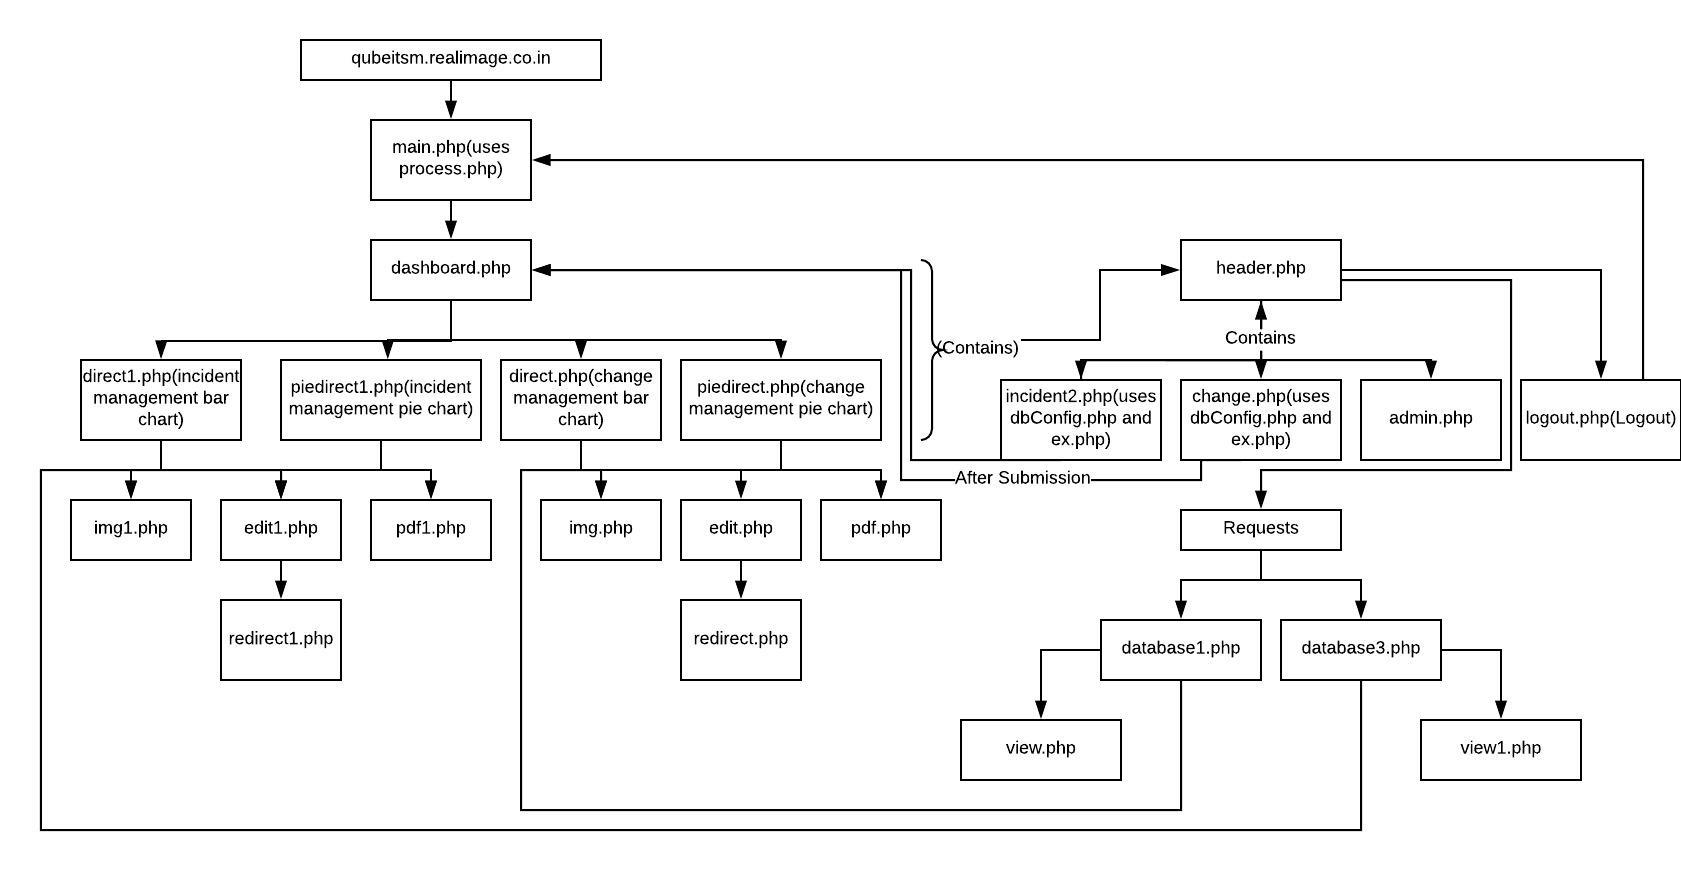
\includegraphics[width=7.0in]{itsm.jpeg}
   
    \label{Flowchart}

\end{center}
\begin{center}

    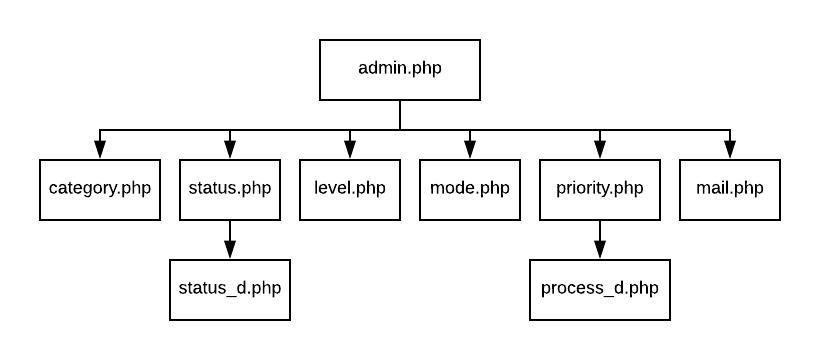
\includegraphics[width=4.0in]{admin.jpeg}
   
    \label{Flowchart}

\end{center}
Note: form.php, incident2.php, redirect.php and redirect1.php requires SMTP configuation, hence uses class.phpmailer.php and class.smtp.php
\section{Details}
\subsection{main.php}
\begin{center}

    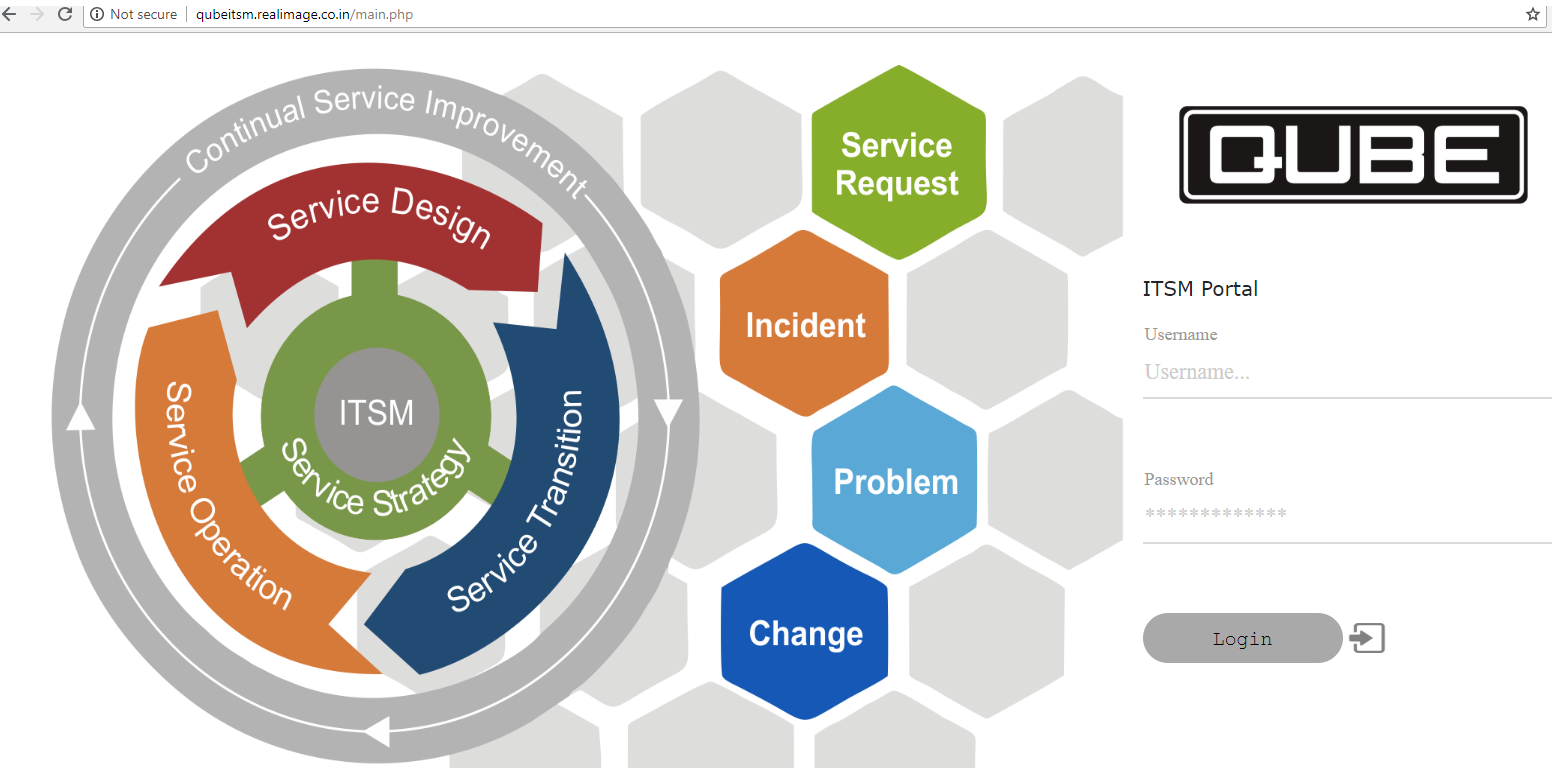
\includegraphics[width=7.0in]{main.png}
   
    \label{}

\end{center}
This is the login page. Special priviledges is given to admin. This is done using the table 'users' where column 'role' is used to assign the priviledge. Only the users with role 'admin' will be able to access the webpages. main.php uses process.php for backend. main.php contains only the front end and the details entered will be taken by process.php and process.php will check for the credentials and redirects the page accordingly. 
\subsection{dashboard.php}
\begin{center}

    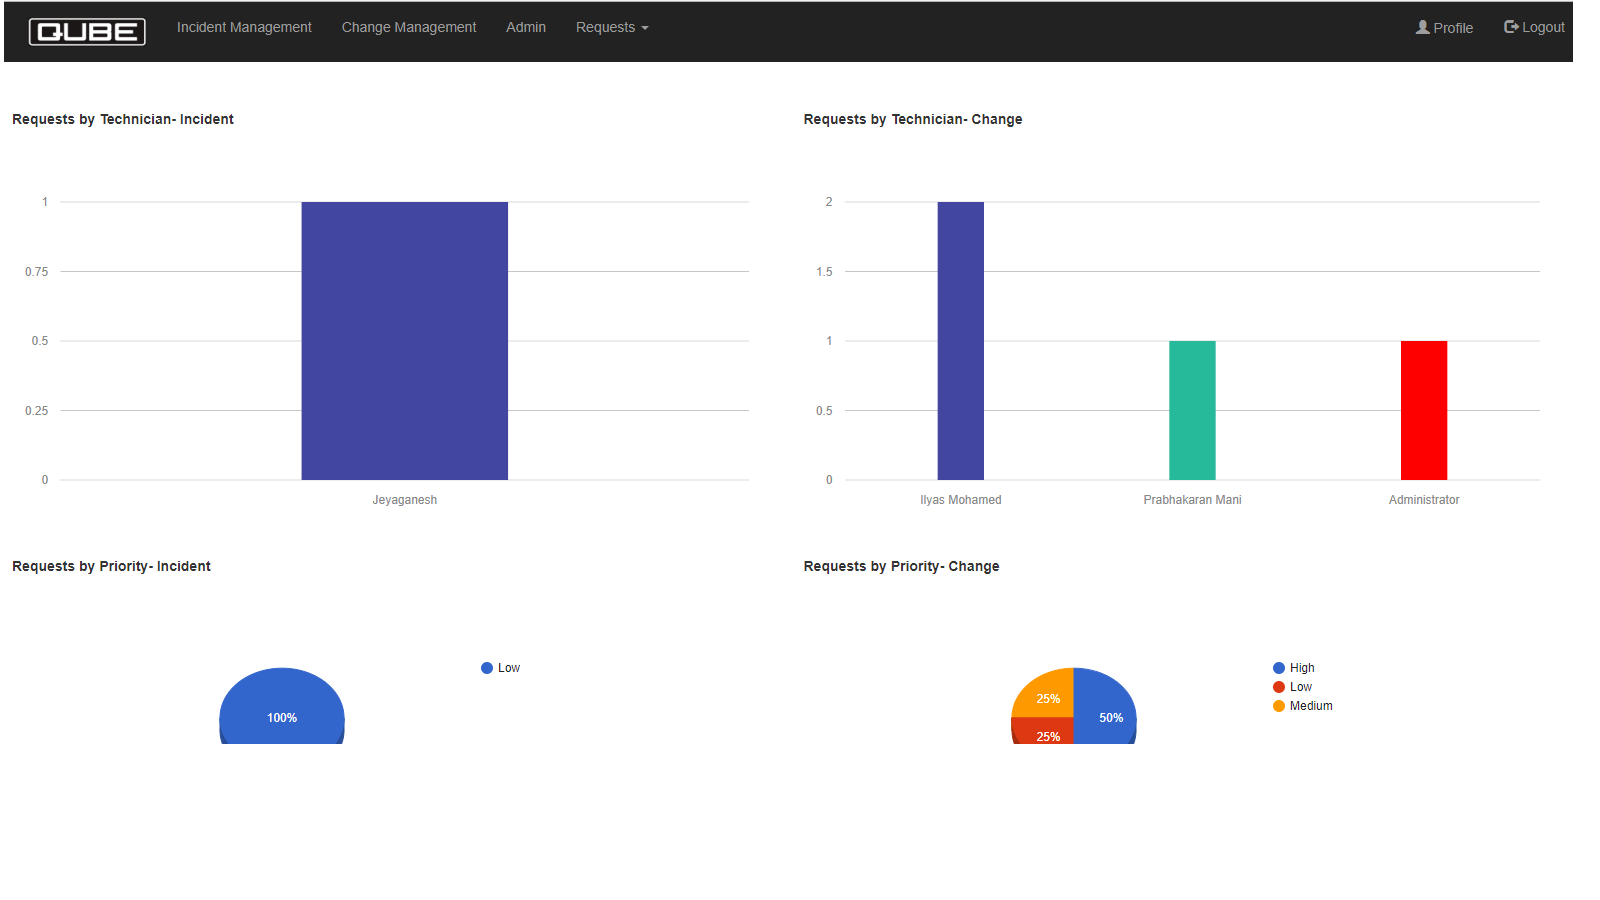
\includegraphics[width=7.0in]{dashboard.png}
   
    \label{}

\end{center}
Dashboard gives the details of the data represented in the form of bar and pie charts. As requests are made respective changes are reflected in the bar and pie charts. For bar charts, morris charts are used and for pie charts, google charts are used. The code for the charts used is javascript. On clicking the data of a chart, it redirects to page based on the data clicked.\\
\big(Note: There are two methods using which you can transfer data from one page to another (GET and POST). GET method is preferred where data entered is not important to be hidden whereas POST method is used when data entered should be hidden.\\ For more details refer: \underline{https://www.w3schools.com/tags/ref\_httpmethods.asp}\big)\\
Here GET method is used when clicking on a particular data in any of the charts. The selected data is transferred to another page (direct.php or direct1.php or piechart.php or piechart1.php ) using GET method.  
\subsection{direct1.php}
\begin{center}

    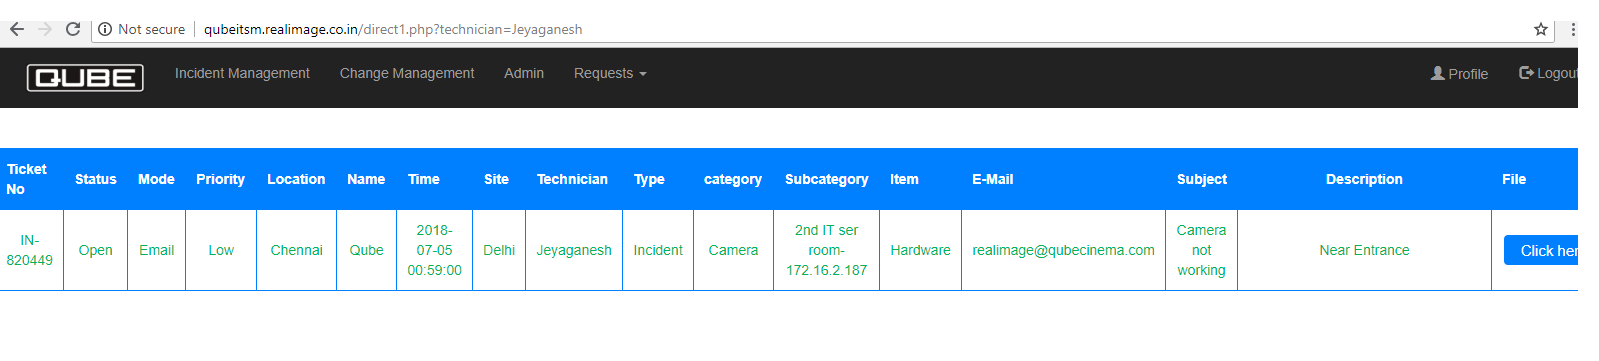
\includegraphics[width=7.0in]{direct1.png}
   
    \label{}

\end{center}
\begin{center}

    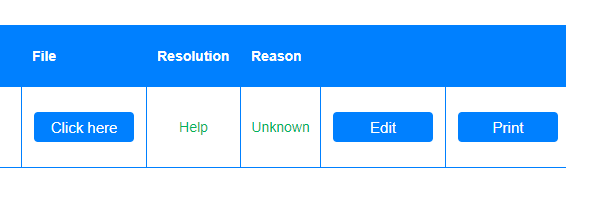
\includegraphics[width=2.0in]{direct1a.png}
   
    \label{}

\end{center}
On Clicking on a data column of Requests by Technician-Incident from dashboard.php, it redirects to direct1.php. From the URL it can be seen that we have used GET method to carry data from one page to another. Click Here button redirects to corresponding image page \big(img1.php\big). Edit button is used to edit the corresponding incident ticket's description, status, priority and technician \big(edit1.php\big). Print is used to print the ticket in PDF format \big(pdf1.php\big). edit1.php, img1.php and pdf1.php uses GET method.
\subsection{direct.php}
\begin{center}

    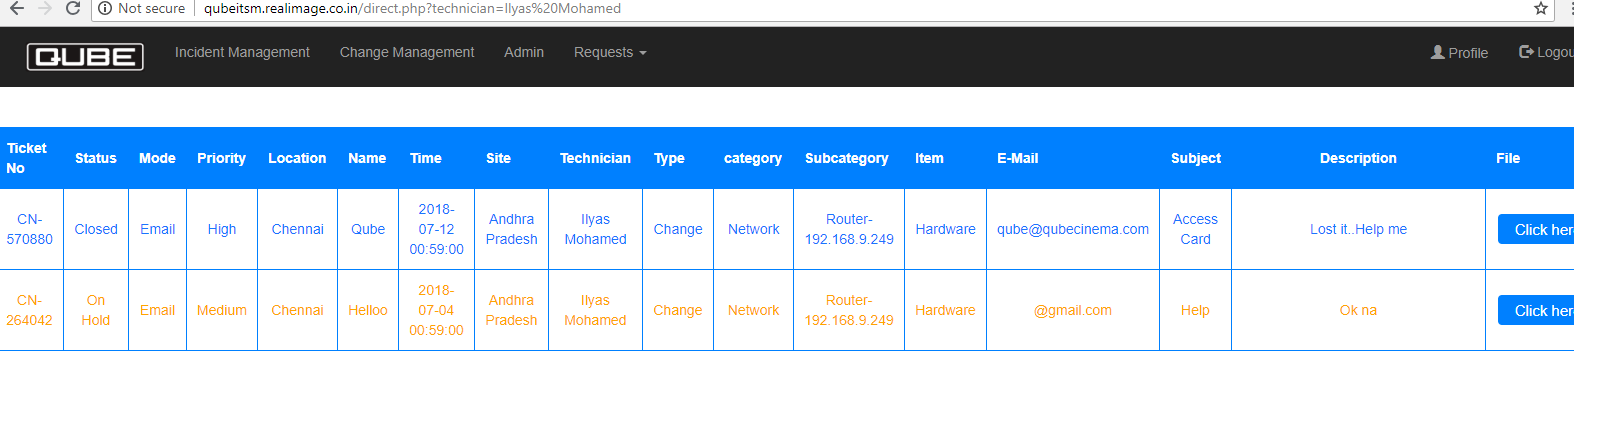
\includegraphics[width=7.0in]{direct.png}
   
    \label{}

\end{center}
On Clicking on a data column of Requests by Technician-Change from dashboard.php, it redirects to direct.php. Click Here button redirects to corresponding image page \big(img.php\big). Edit button is used to edit the corresponding incident ticket's description, status, priority and technician \big(edit.php\big). Print is used to print the ticket in PDF format \big(pdf.php\big). edit.php, img.php and pdf.php uses GET method.\\
\big(Note: To see Edit and Print button scroll towards right in webpage\big).
\subsection{piedirect1.php}
\begin{center}

    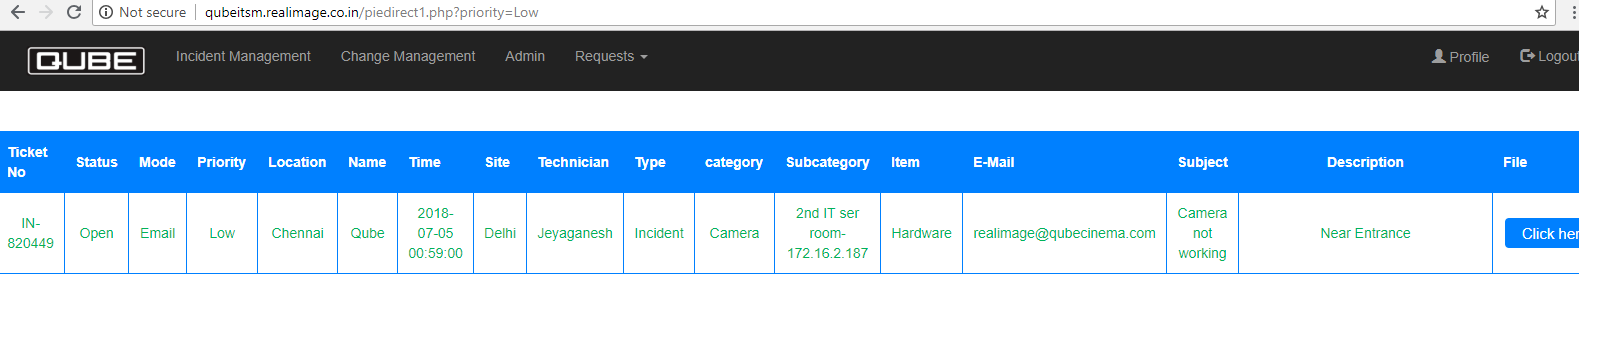
\includegraphics[width=7.0in]{piedirect1.png}
   
    \label{}

\end{center}
On Clicking on any data of Requests by Priority-Incident piechart from dashboard.php, it redirects to piedirect1.php. Click Here button redirects to corresponding image page \big(img1.php\big). Edit button is used to edit the corresponding incident ticket's description, status, priority and technician \big(edit1.php\big). Print is used to print the ticket in PDF format \big(pdf1.php\big). edit1.php, img1.php and pdf1.php uses GET method.\\
\big(Note: To see Edit and Print button scroll towards right in webpage\big).

\subsection{piedirect.php}
\begin{center}

    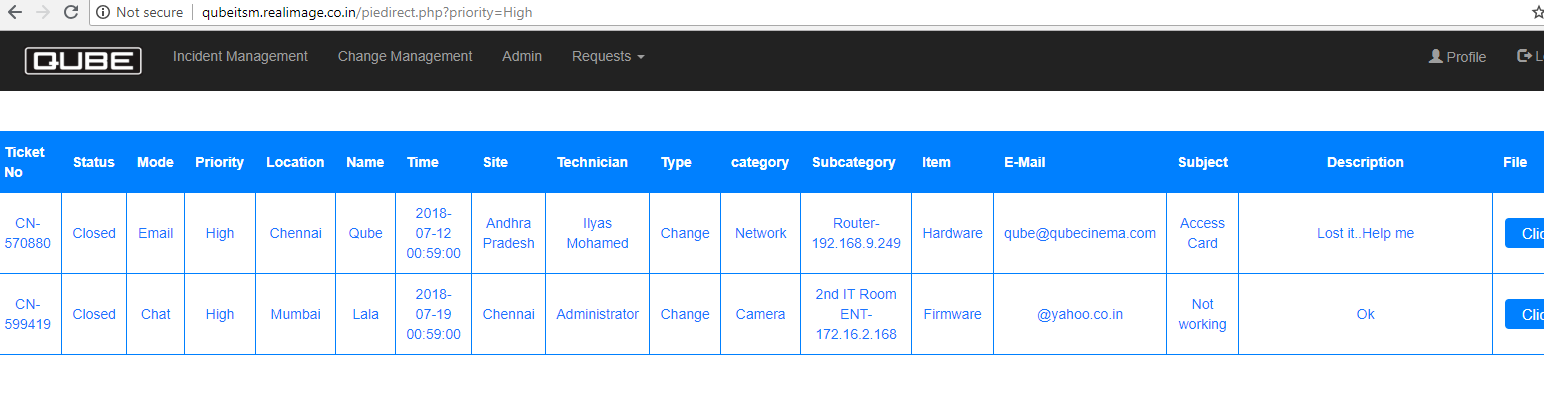
\includegraphics[width=7.0in]{piedirect.png}
   
    \label{}

\end{center}
On Clicking on any data of Requests by Priority-Change piechart from dashboard.php, it redirects to piedirect.php. Click Here button redirects to corresponding image page \big(img.php\big). Edit button is used to edit the corresponding incident ticket's description, status, priority and technician \big(edit.php\big). Print is used to print the ticket in PDF format \big(pdf.php\big). edit.php, img.php and pdf.php uses GET method.\\
\big(Note: To see Edit and Print button scroll towards right in webpage\big).
\subsection{img.php/img1.php}
\begin{center}

    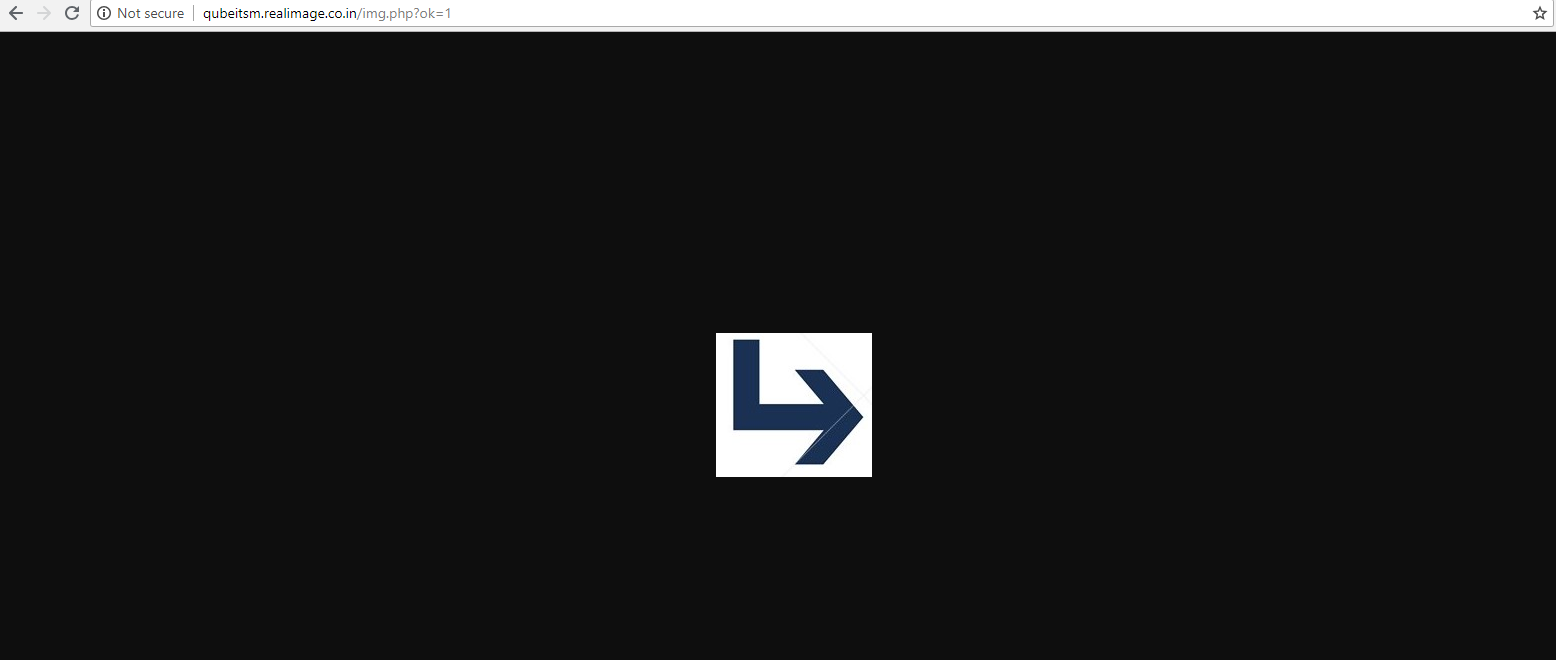
\includegraphics[width=7.0in]{img.png}
   
    \label{}

\end{center}
img.php is for change management and img1.php is for incident management. On clicking the Click here button from any of direct.php or piedirect.php or database1.php or view.php redirects to img.php of change management displaying the corresponding image of the ticket. Similarly, On clicking the Click here button from any of direct1.php or piedirect1.php or database3.php or view1.php redirects to img1.php of incident management displaying the corresponding image of the ticket.
\subsection{edit.php/edit1.php}
\begin{center}

    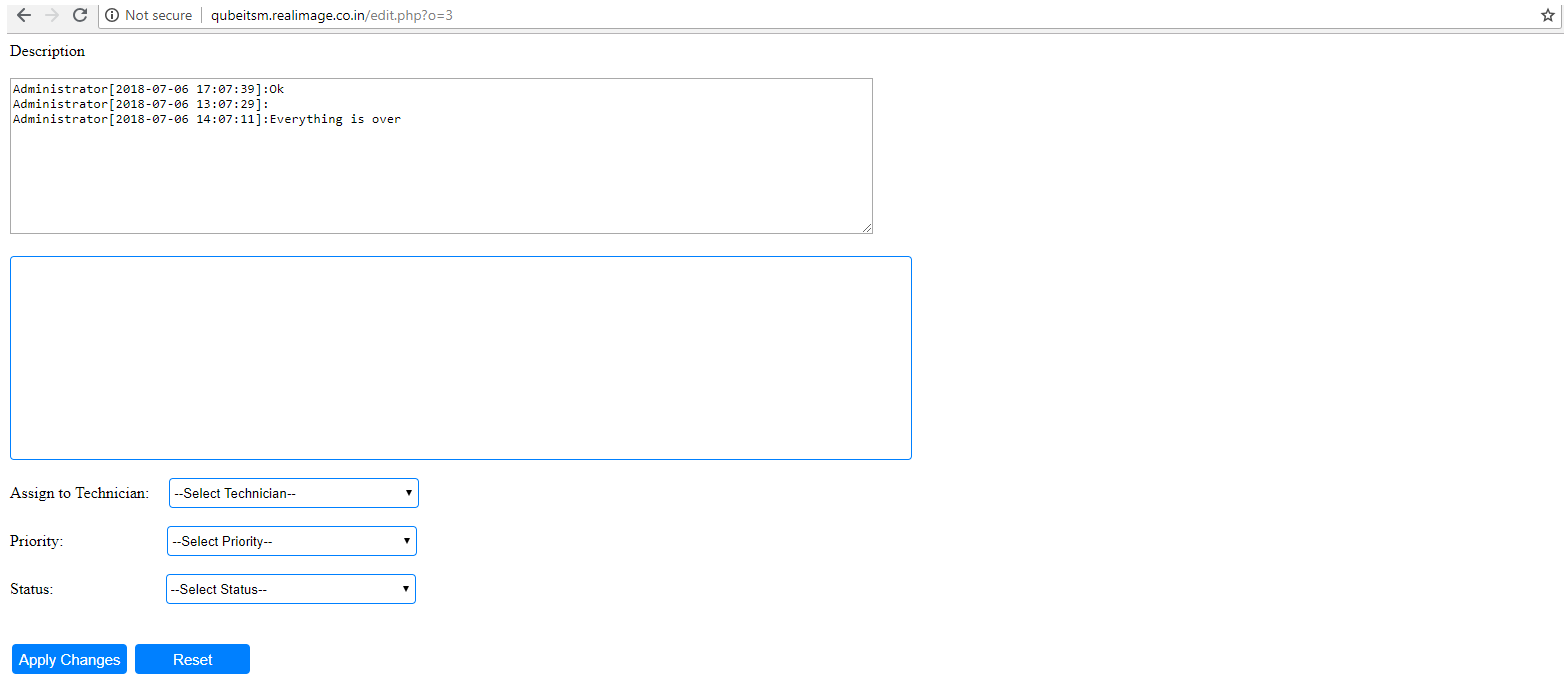
\includegraphics[width=7.0in]{edit.png}
   
    \label{}

\end{center}
edit.php is for change management and edit1.php is for incident management. On clicking the Edit button from any of direct.php or piedirect.php or database1.php or view.php redirects to edit.php of change management. Similarly, On clicking the Edit button from any of direct1.php or piedirect1.php or database3.php or view1.php redirects to edit1.php of incident management. Both edit.php and edit1.php has description text area, status, priority and technician drop down list.
First description text area is readonly, it contains the description written by each technician to whom it is assigned along with the timestamp. Second description text box is for the technician to update the content. Status and Priority can be changed and the changes will be reflected in the corresponding database table. After a technician is done with his work, he can assign the ticket to someother technician which will be alerted to the other technician via e-mail. edit.php uses redirect.php which contains queries and php code for updating the changes made. Similarly, edit1.php uses redirect1.php.

\subsection{pdf.php/pdf1.php}
\begin{center}

    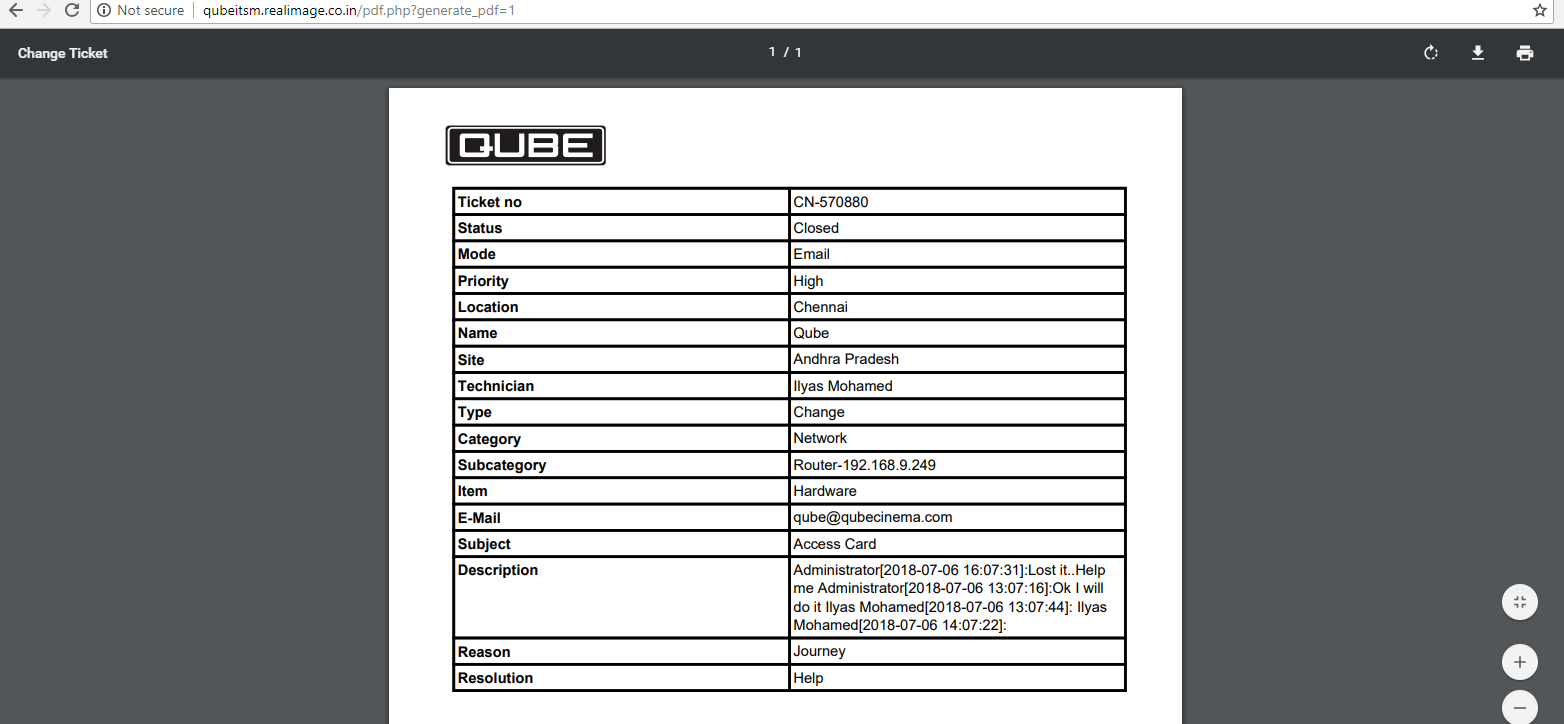
\includegraphics[width=7.0in]{pdf.png}
   
    \label{}

\end{center}
pdf.php is for change management and pdf1.php is for incident management. On clicking the Print button from any of direct.php or piedirect.php or database1.php or view.php redirects to pdf.php of change management. Similarly, On clicking the Print button from any of direct1.php or piedirect1.php or database3.php or view1.php redirects to pdf1.php of incident management. TCPDF software is used to view the contents in the form of pdf. Before working with PDF, tcpdf folder downloaded from net must be saved in your website folder. 
\subsection{dbConfig.php}
PHP code for database connection with localhost.
\subsection{header.php}
\begin{center}

    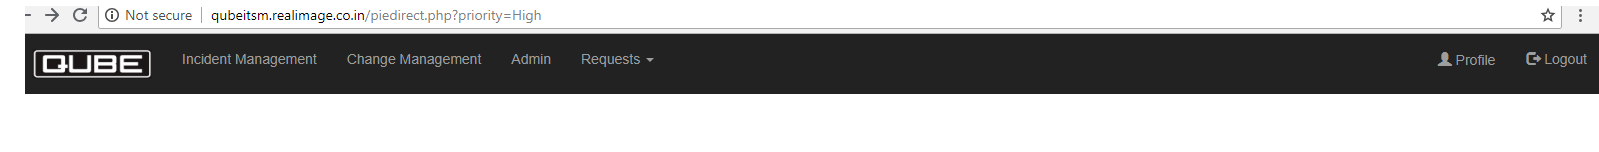
\includegraphics[width=7.0in]{header.png}
   
    \label{}

\end{center}
header.php is included almost in all webpages to easily direct to a webpage. Clicking on the Qube logo directs to dashboard.php. Incident Management directs to incident2.php. Change Management directs to form.php. Admin directs to admin.php. Requests contains drop down list which contains incident and change requests details made so far. On placing the mouse over Profile, it shows the user who logged in and logout is used to log out of the website.
\subsection{incident2.php}
\begin{center}

    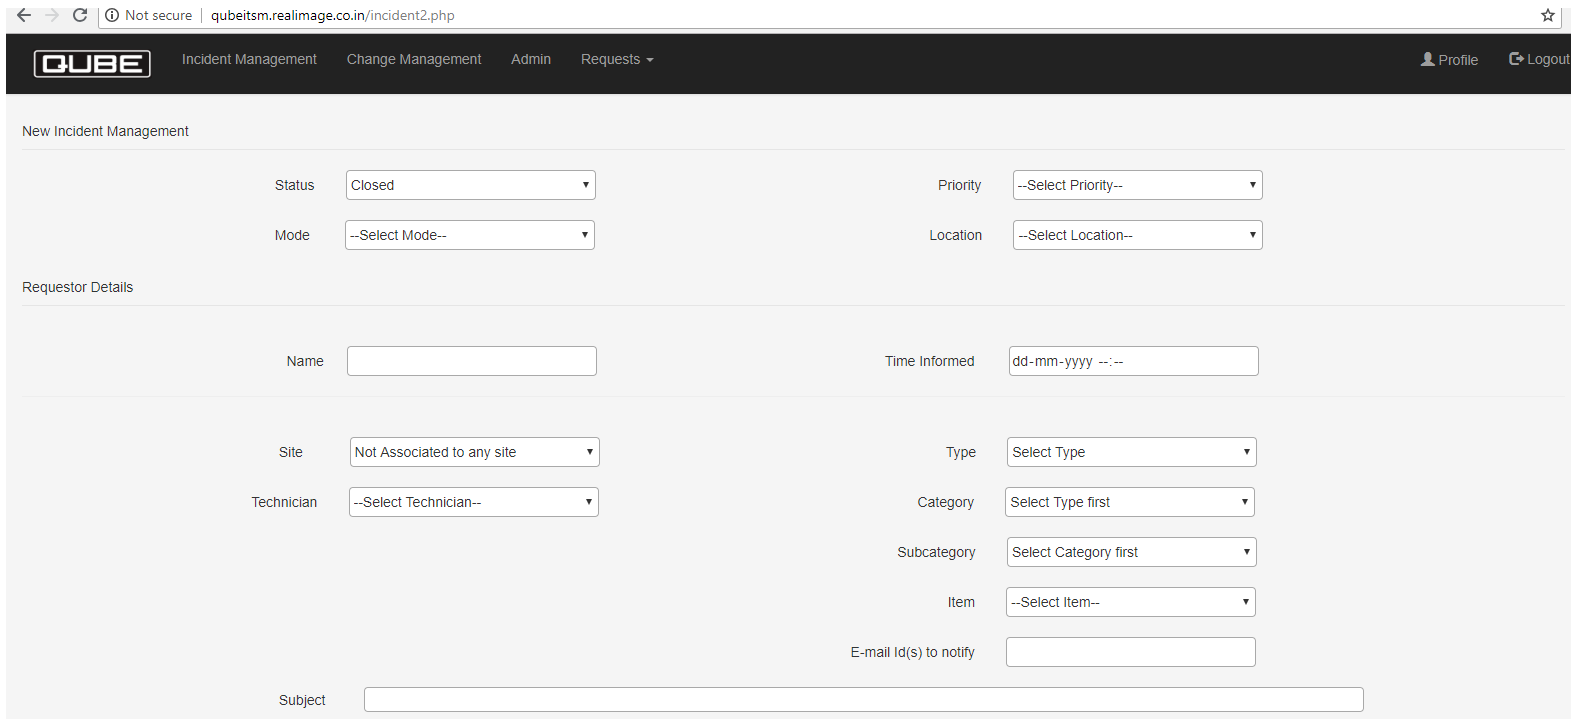
\includegraphics[width=7.0in]{incident.png}
   
    \label{}

\end{center}
\begin{center}

    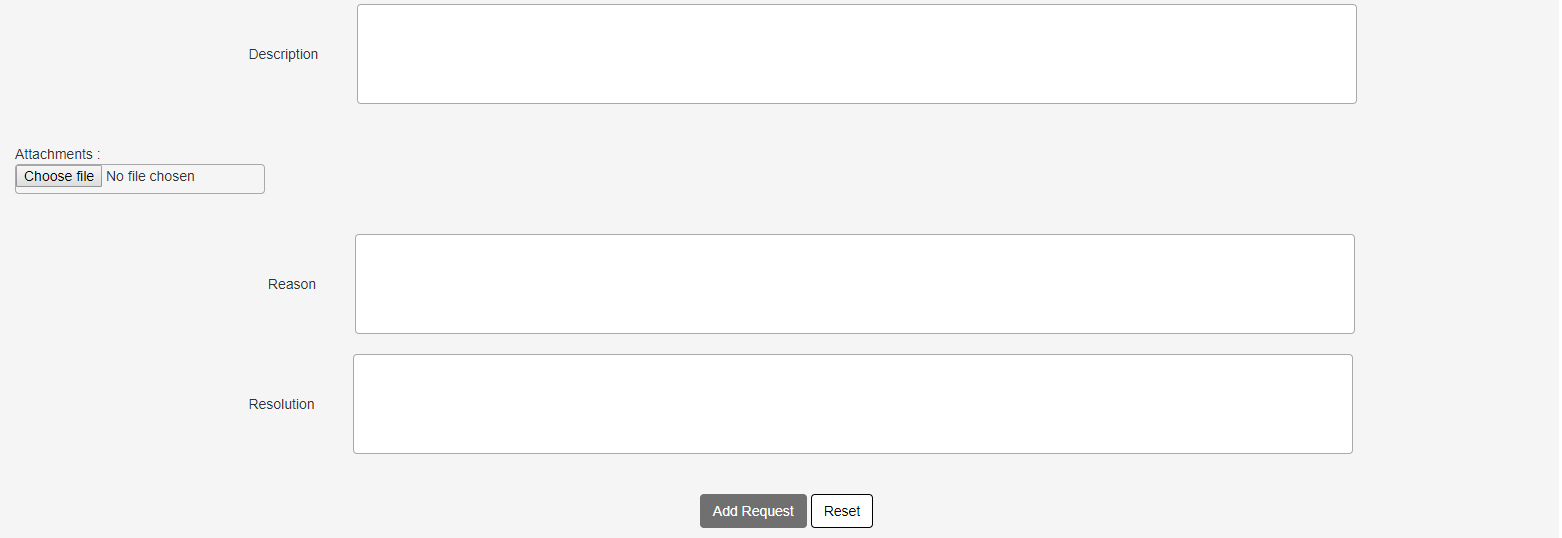
\includegraphics[width=7.0in]{incident1.png}
   
    \label{}

\end{center}
After entering the details, Add Request button is clicked and a new ticket is raised and stored in database table incident. The corresponding Technician receives the mail in pdf format. Email is configured using SMTP protocol. Then you will be redirected to dashboard.php\\
\big(Note: Make sure you have class.phpmailer.php and class.smtp.php inside your website folder\big).
\begin{center}

    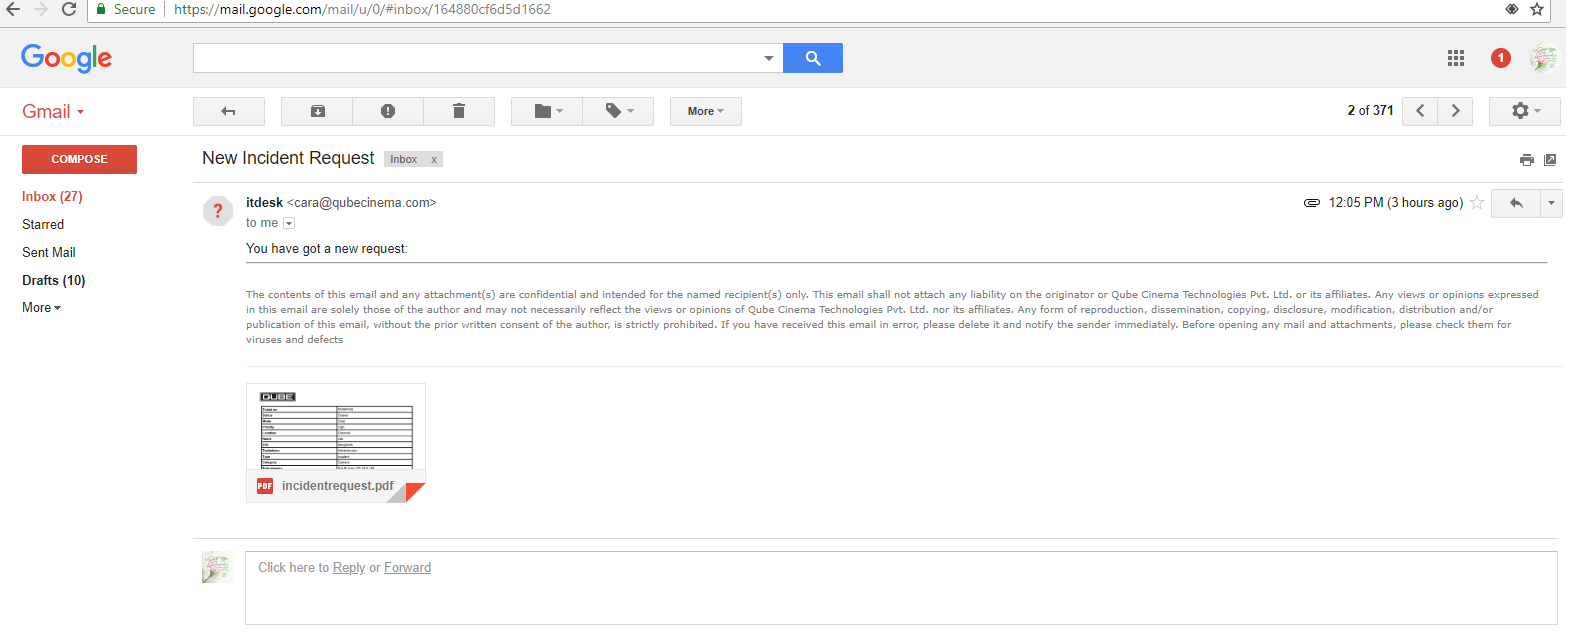
\includegraphics[width=7.0in]{mail.png}
   
    \label{}

\end{center}
\subsection{form.php}
\begin{center}

    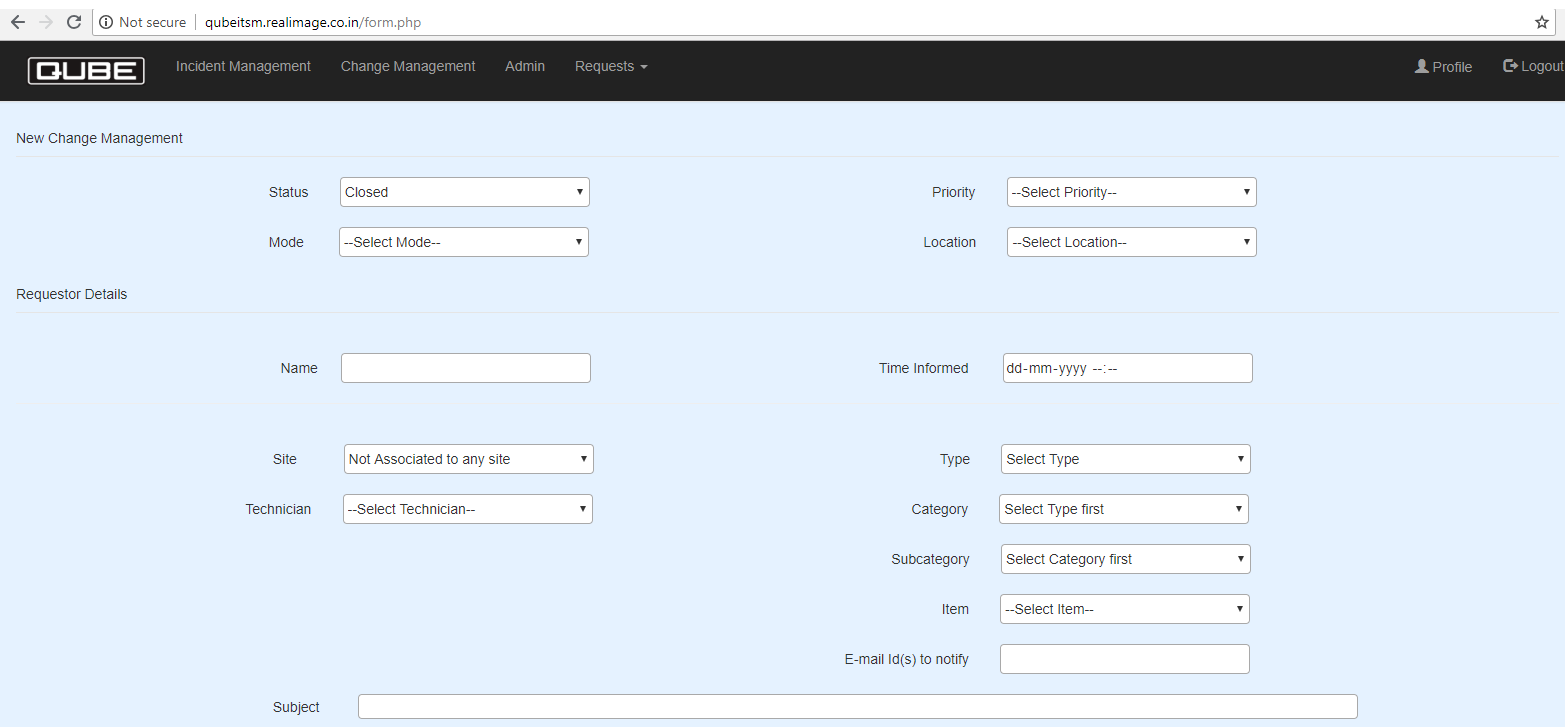
\includegraphics[width=7.0in]{form.png}
   
    \label{}

\end{center}
After entering the details, Add Request button is clicked and a new ticket is raised and stored in database table change1. The corresponding Technician receives the mail in pdf format. Email is configured using SMTP protocol. Then you will be redirected to dashboard.php.\\
\big(Note: Make sure you have class.phpmailer.php and class.smtp.php inside your website folder\big).
\subsection{admin.php}
\begin{center}

    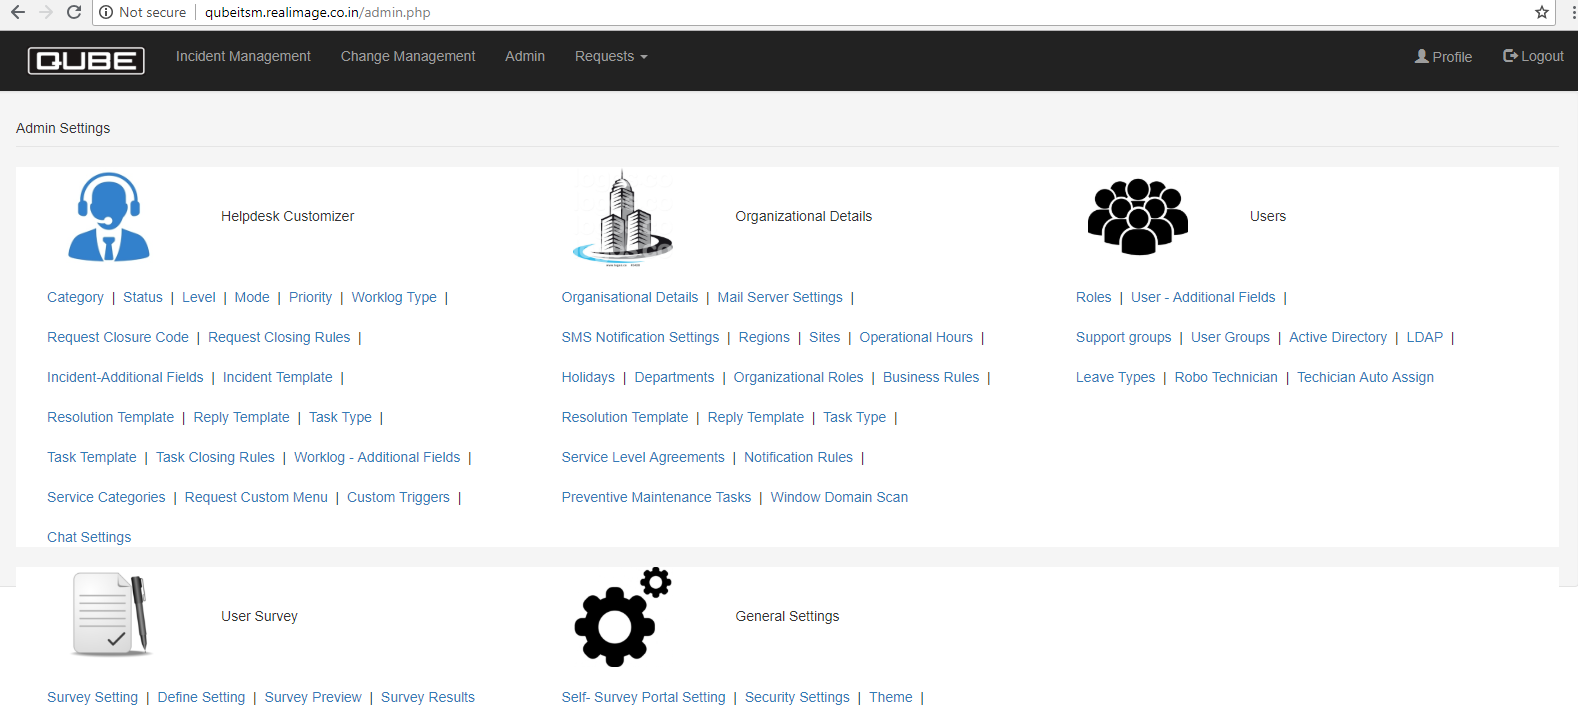
\includegraphics[width=7.0in]{admin.png}
   
    \label{}

\end{center}
\subsection{database1.php/database3.php}
\begin{center}

    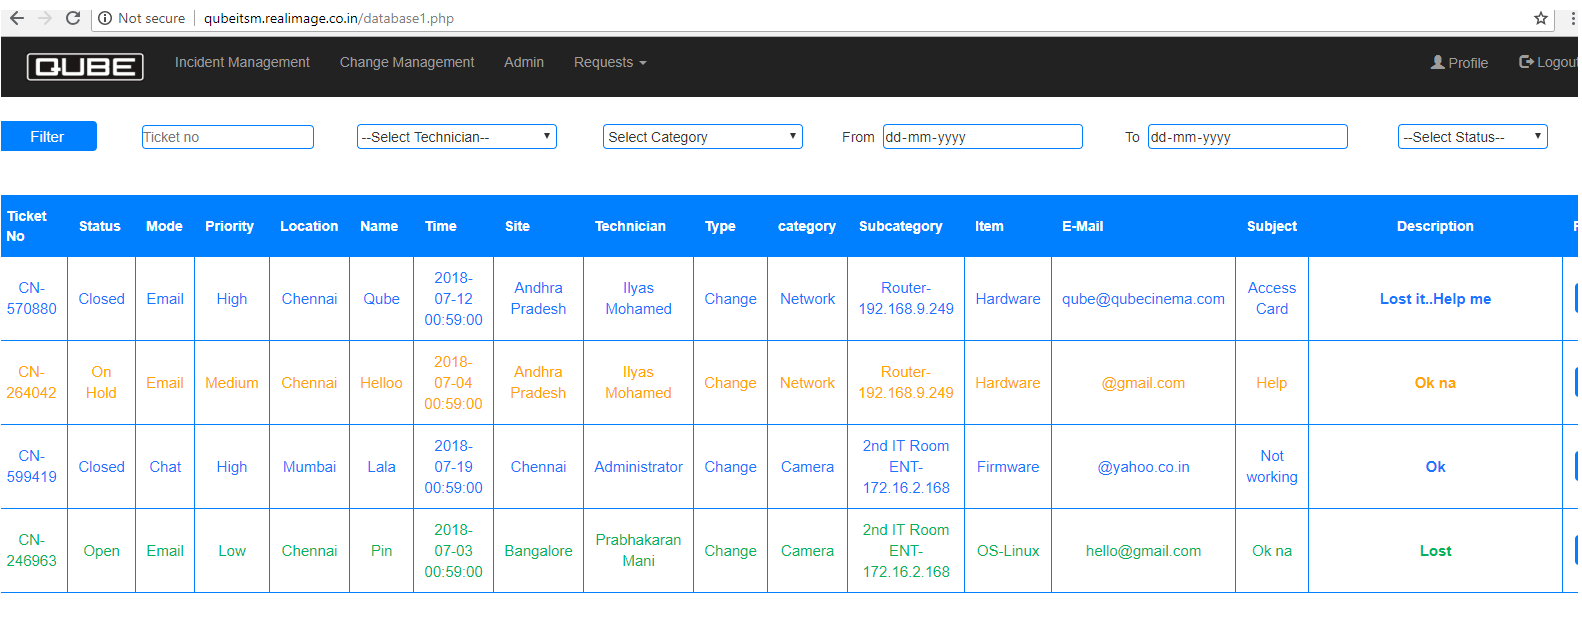
\includegraphics[width=7.0in]{database.png}
   
    \label{}

\end{center}
database1.php contains details of change requests and database3.php contains details of incident requests made.\\
Status with Closed Requests are marked with blue color\\
High priority requests are marked with red color\\
Low priority requests are marked with green color\\
Medium priority requests are marked with yellow color.\\
In the beginning of the page you can filter the details based on Technician, Ticketno, Category, Technician and Category and based on period and status \big(ex. last 20 days Closed requests\big). The filtered details uses view.php for change tickets and view1.php for incident tickets.\\
\big(Note: To see Click Here, Edit and Print button scroll towards right in webpage\big).
\subsection{view.php/view1.php}
\subsubsection{Based on Technician, Ticketno, Category, Technician and Category}
\begin{center}

    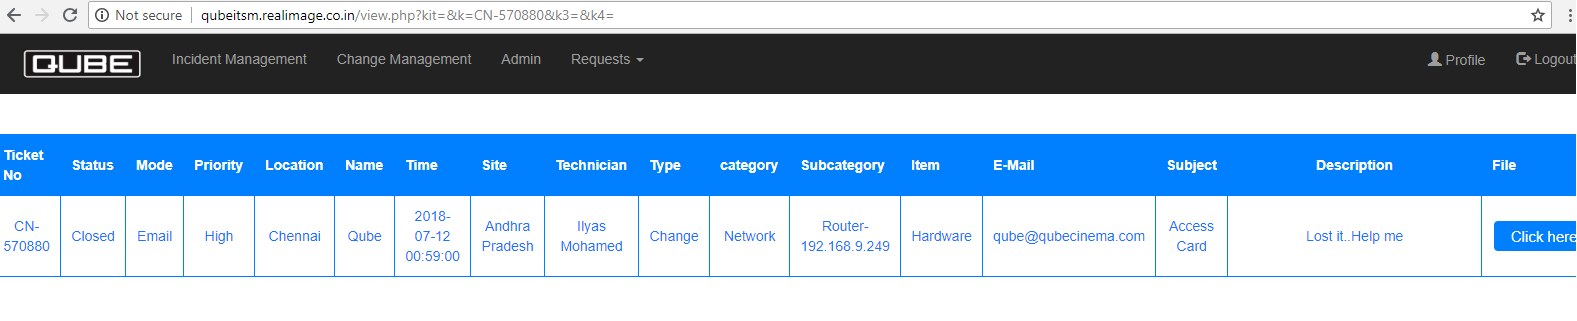
\includegraphics[width=7.0in]{view.png}
   
    \label{}

\end{center}
view.php and view1.php uses GET method.On Filtering based on the above mentioned criteria we can see the filtered details.\\
\big(Note: To see Edit and Print button scroll towards right in webpage\big).
\subsubsection{Based on period and status}
\begin{center}

    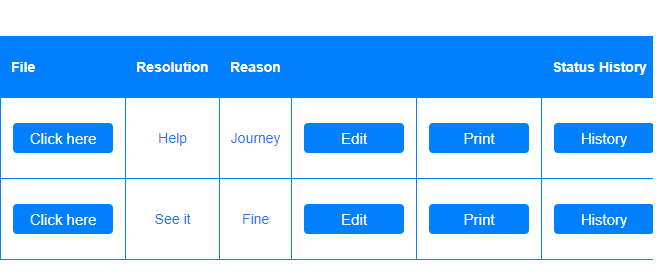
\includegraphics[width=3.0in]{view1.png}
   
    \label{}

\end{center}
On filtering based on the mentioned criteria we can see the details of the past x days Closed/Open/.. tickets. It has one extra Status History Field which on Click takes to history.php which also uses GET method.
\begin{center}

    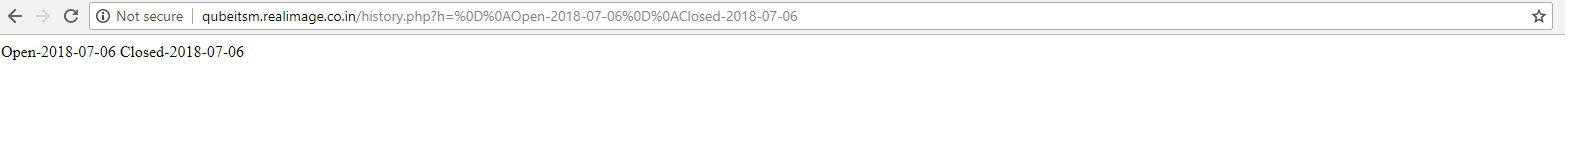
\includegraphics[width=7.0in]{history.png}
   
    \label{}

\end{center}
\subsection{category.php}
\begin{center}

    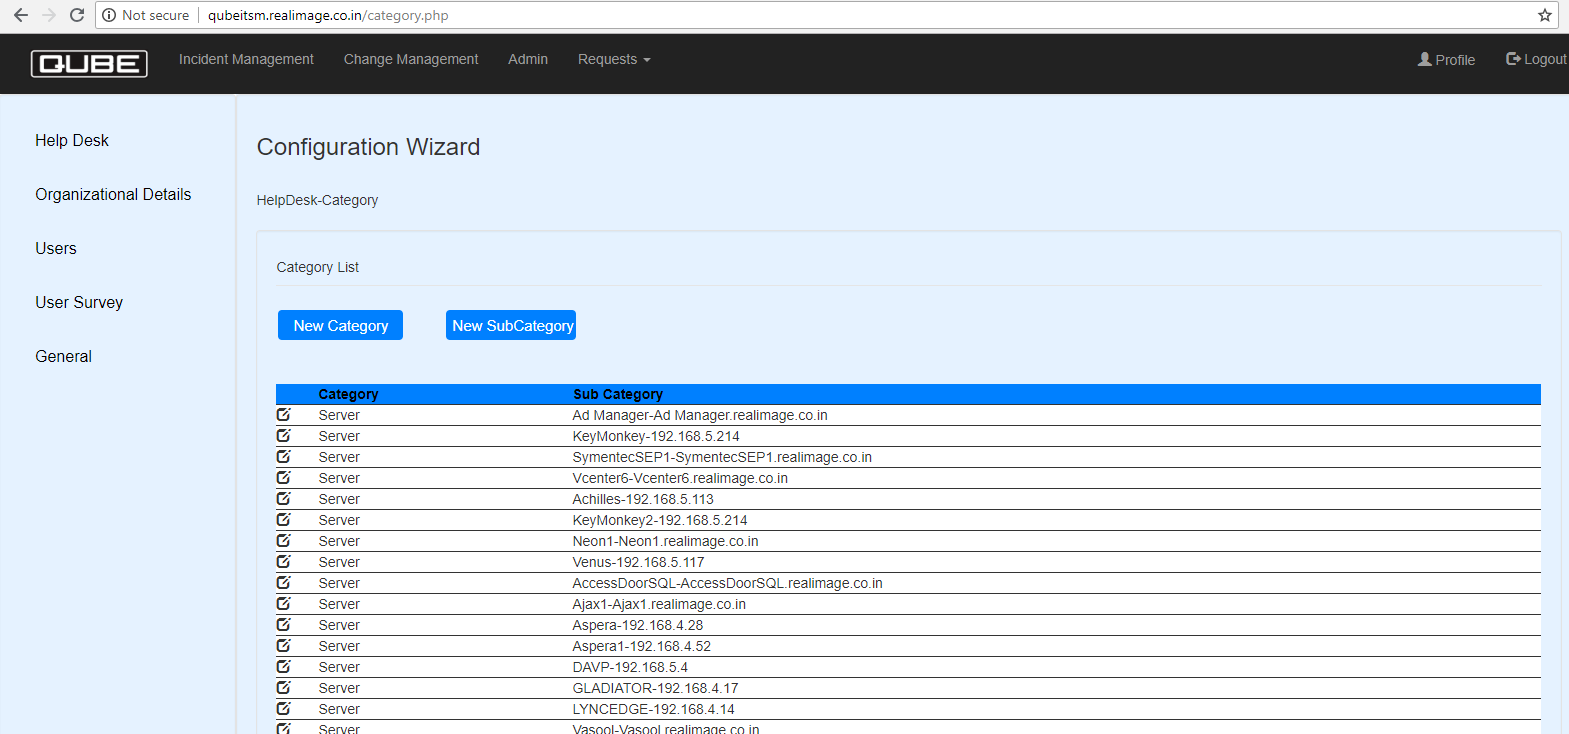
\includegraphics[width=7.0in]{category.png}
   
    \label{}

\end{center}
In admin.php on clicking Category link, it directs to category.php. Here we can add New category and subcategory and changes will be made in category and subcategory tables.
\subsection{status.php}
\begin{center}

    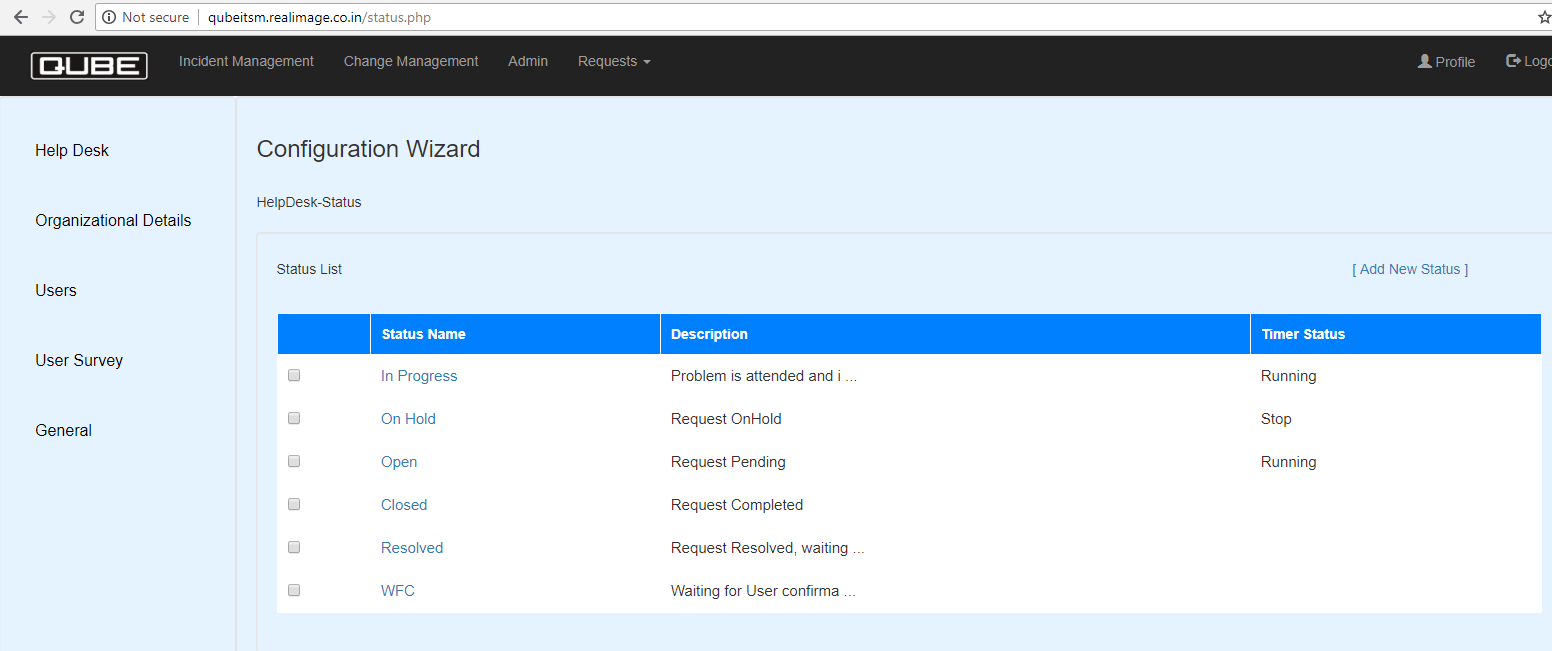
\includegraphics[width=7.0in]{status.png}
   
    \label{}

\end{center}
In admin.php on clicking Status link, it directs to status.php. To add a New Status, click on the link [ Add New Status ] present at the rightmost corner. The newly added status will be reflected in the table statuslist.
\begin{center}

    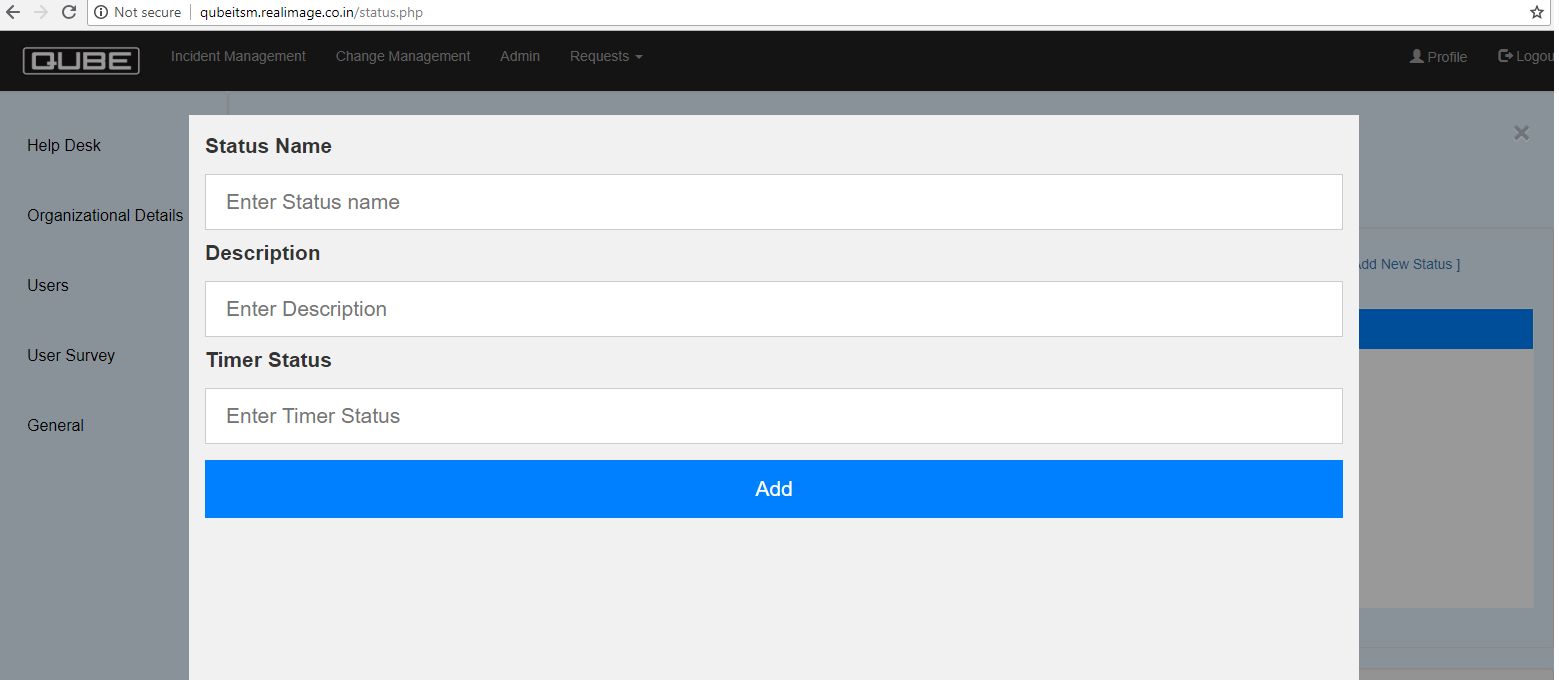
\includegraphics[width=7.0in]{status2.png}
   
    \label{}

\end{center}

To view incident and change tickets of each status, click on the link of Status Name and it directs to status\_d.php which uses GET method to retrieve data.
\begin{center}

    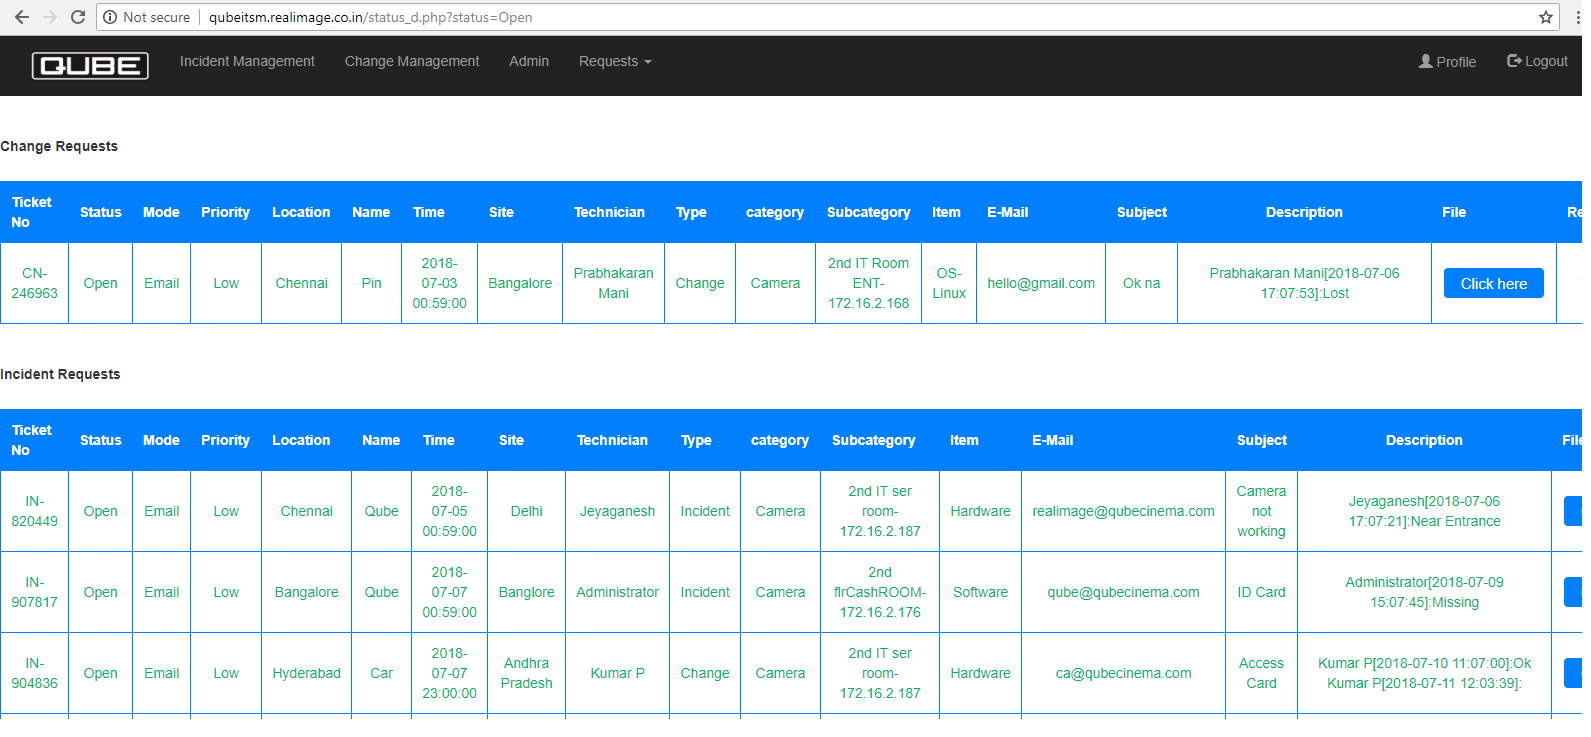
\includegraphics[width=7.0in]{status1.png}
   
    \label{}

\end{center}
\subsection{level.php}
\begin{center}

    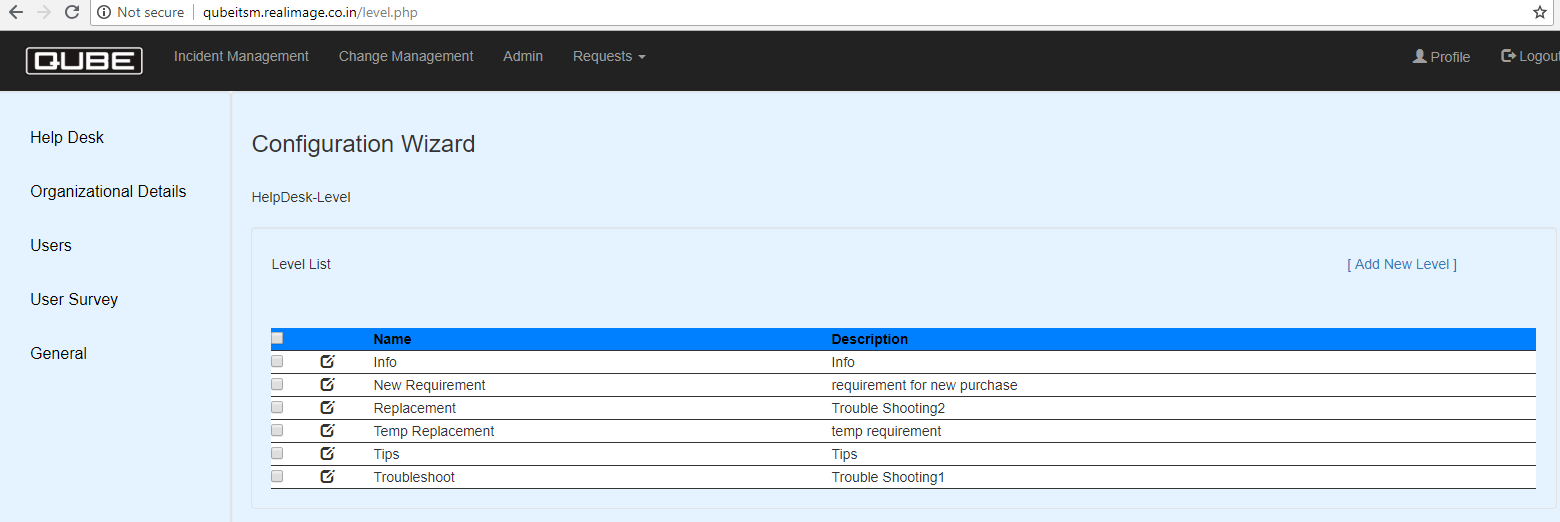
\includegraphics[width=7.0in]{level.png}
   
    \label{}

\end{center}
In admin.php on clicking Level link, it directs to level.php. 
\subsection{mode.php}
\begin{center}

    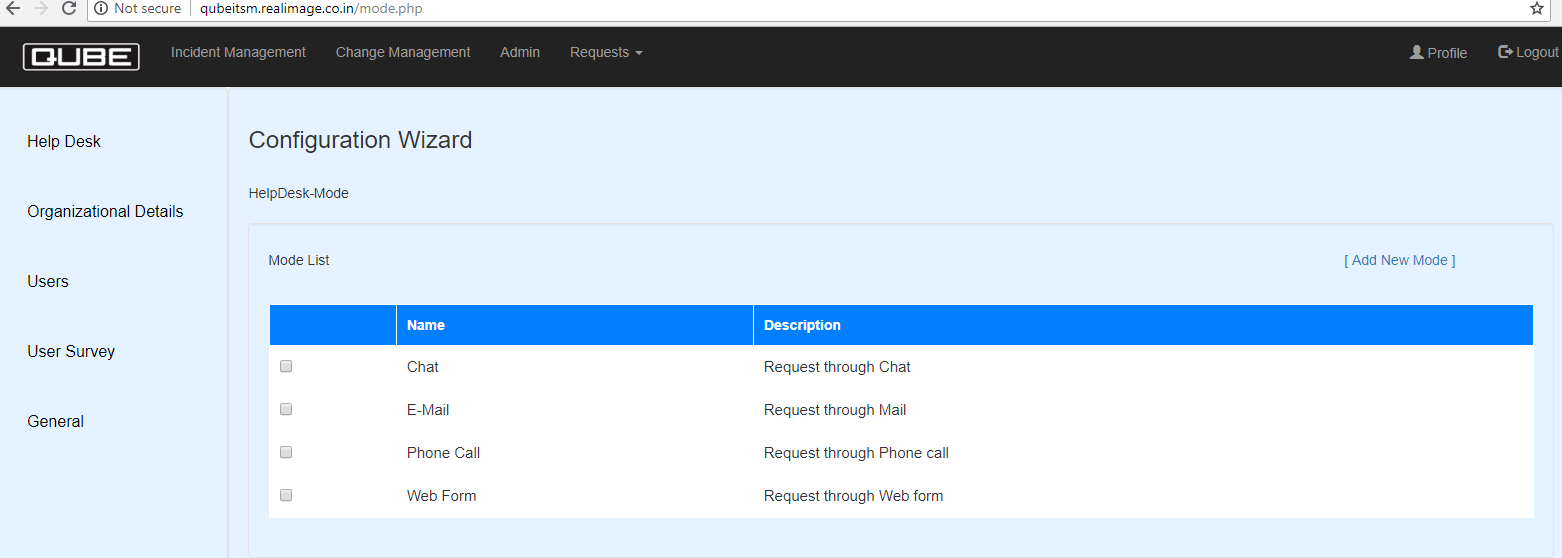
\includegraphics[width=7.0in]{mode.png}
   
    \label{}

\end{center}
In admin.php on clicking Mode link, it directs to mode.php. To add a New Mode, click on the link [ Add New Mode ] present at the rightmost corner. The newly added mode will be reflected in the table modelist.
\subsection{priority.php}
\begin{center}

    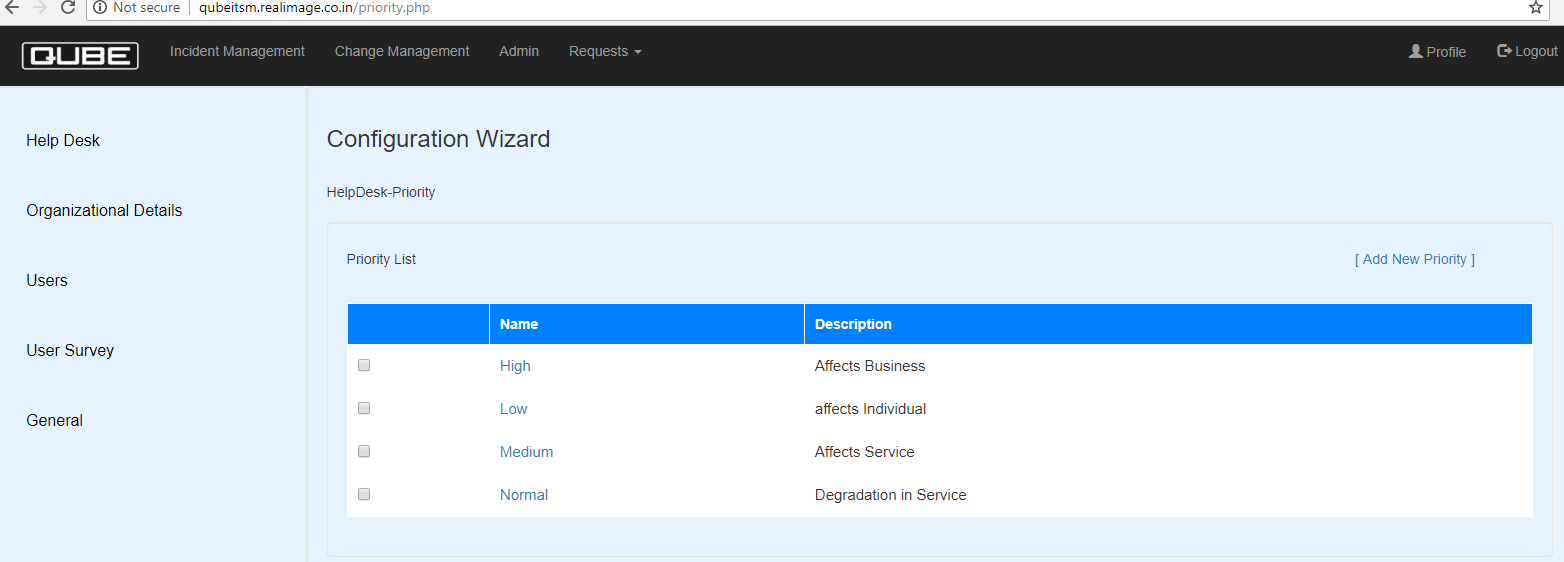
\includegraphics[width=7.0in]{priority.png}
   
    \label{}

\end{center}
In admin.php on clicking Priority link, it directs to priority.php. To add a New priority, click on the link [ Add New Priority ] present at the rightmost corner. The newly added priority will be reflected in the table prioritylist. To view incident and change tickets of each priority, click on the link of column Name and it directs to priority\_d.php which uses GET method to retrieve data.
\begin{center}

    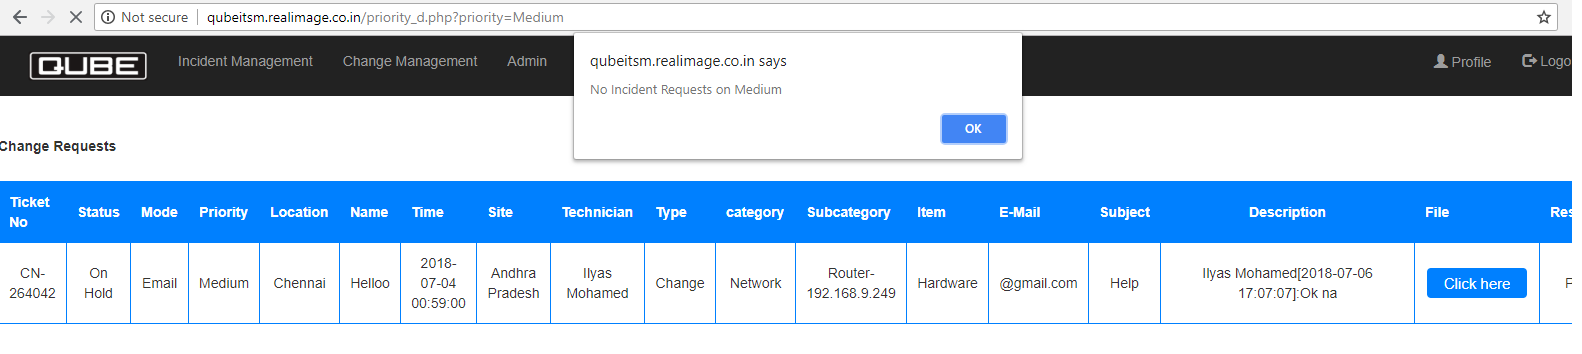
\includegraphics[width=7.0in]{priority1.png}
   
    \label{}

\end{center} 
 \subsection{mail.php}
\begin{center}

    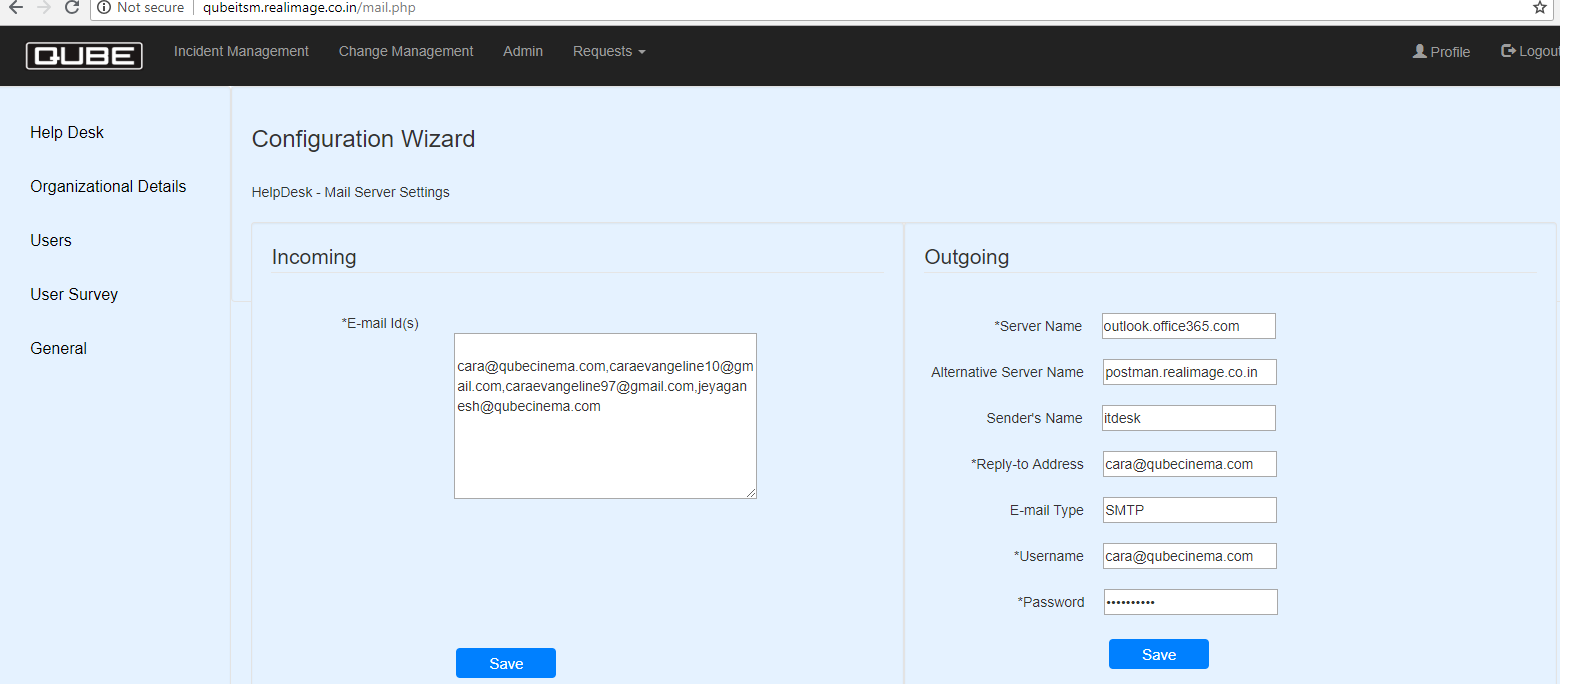
\includegraphics[width=7.0in]{mail1.png}
   
    \label{}

\end{center}
In admin.php on clicking Mail Server Settings link, it directs to mail.php. Here we can configure the mail through which all mails are sent and you can add mail ids to which you must receive the tickets. For every technician, incoming E-mail id\big(s\big) can be added according to the technician's wish. Alert through mail of the ticket allotted to a technician will be sent to the all the mail ids given by the technician in Incoming E-mail ids field. 
\section{References}
Few main references are as below:\\\\
1.https://www.w3schools.com/pHP/default.asp\\
2.https://www.w3schools.com/Css/\\
3.https://www.w3schools.com/htmL/\\
4.https://www.w3schools.com/jS/default.asp\\
5.https://www.quackit.com/php/tutorial/php\_mail\_configuration.cfm
\end{document}
